\begin{figure}[H]
    \centering
    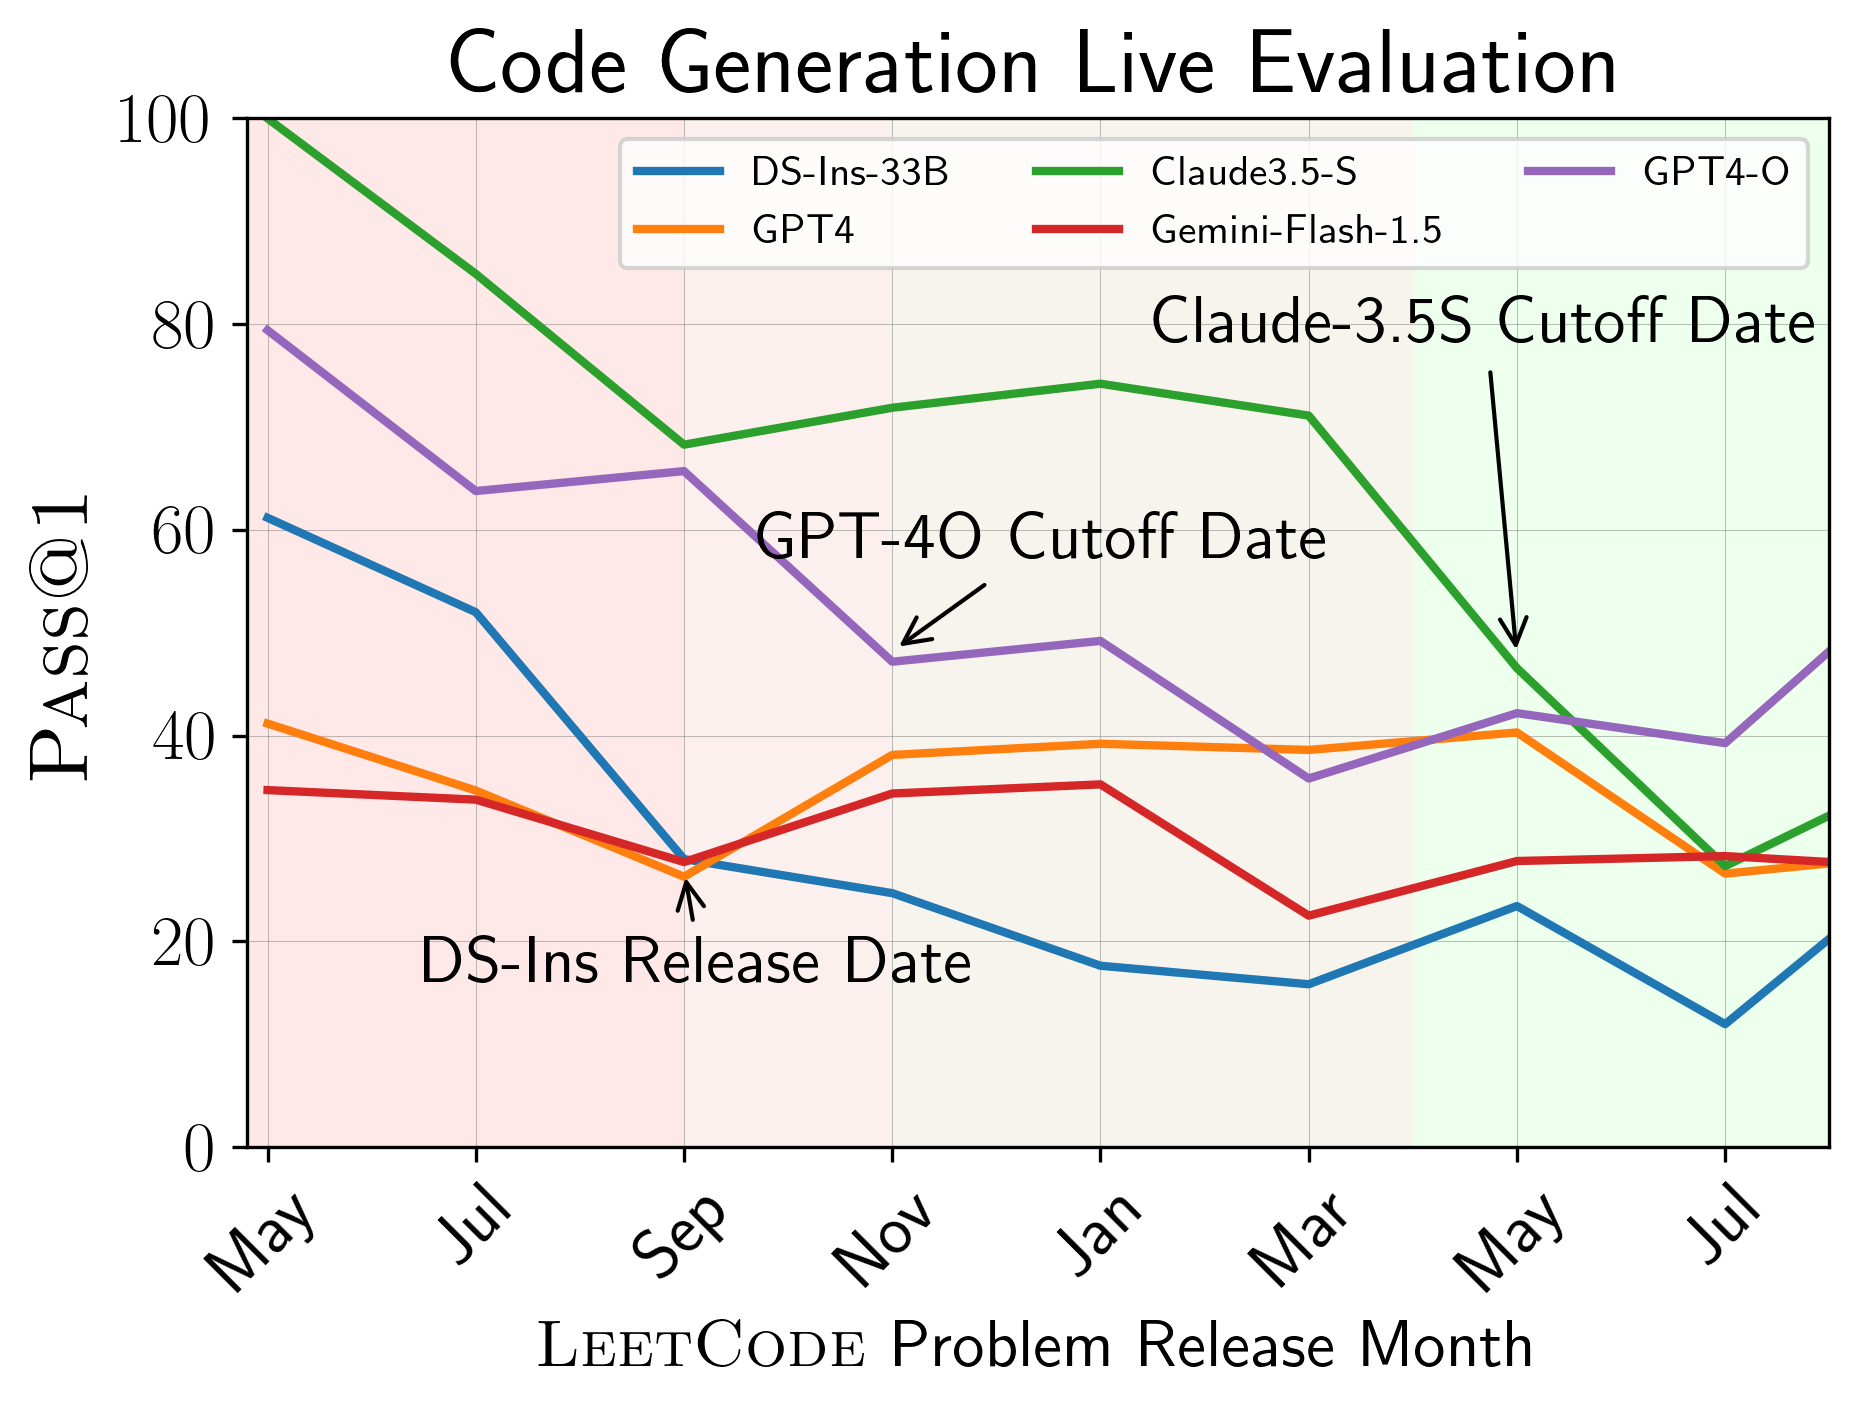
\includegraphics[width=0.49\linewidth]{figures/contamination_new/main_20_codegen_leetcode.png}
    \hfil
    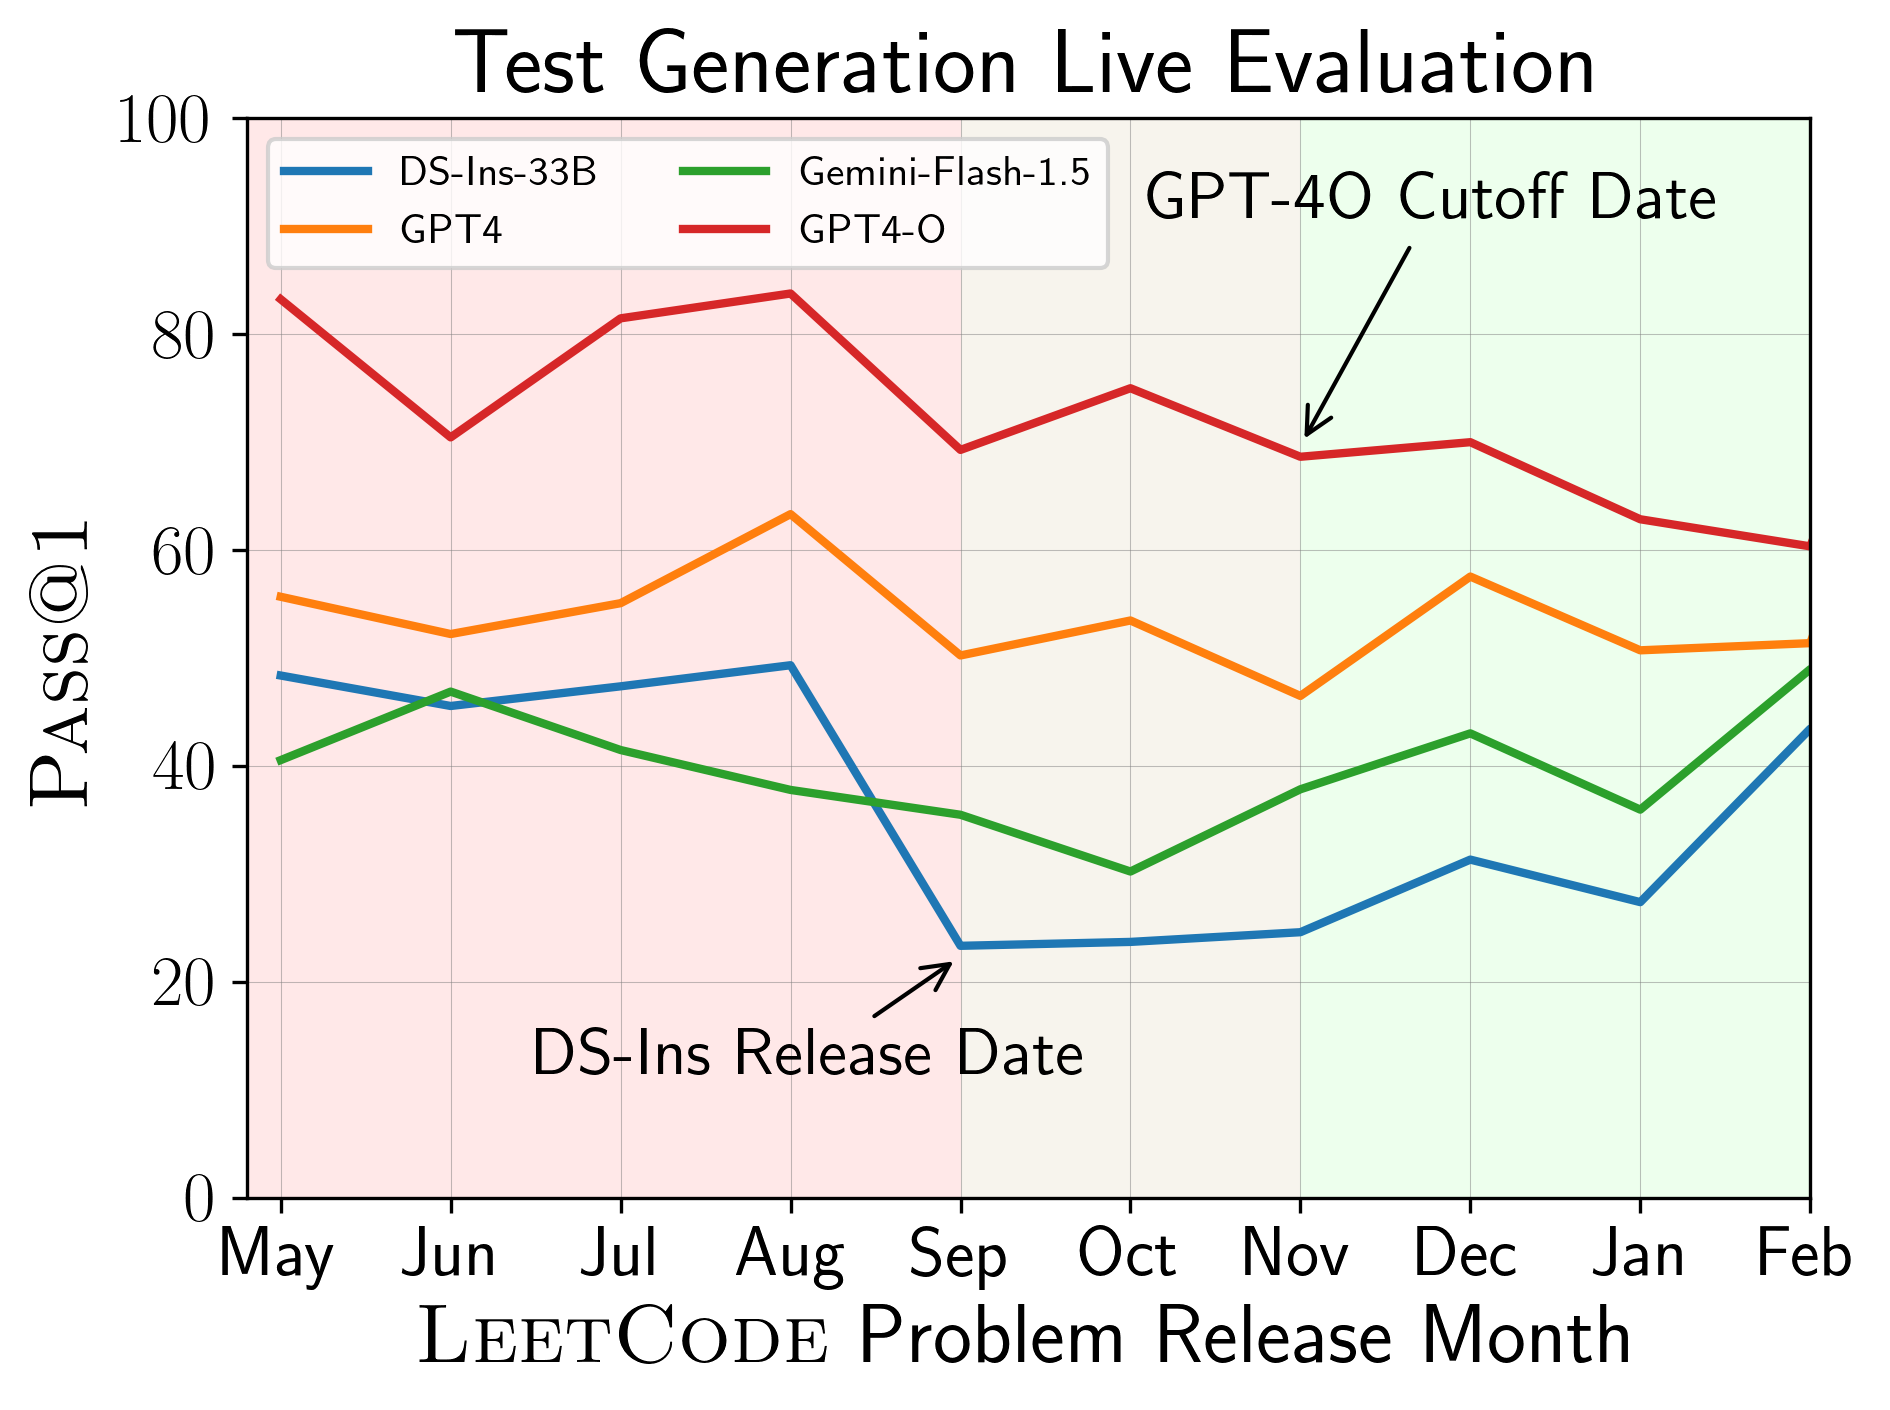
\includegraphics[width=0.49\linewidth]{figures/contamination_new/main_14_testgen_leetcode.png}

    \caption{
        \livecodebench{} comprises problems marked with release dates, allowing evaluations over different time windows.
        The code-generation and test-output-prediction panels depict performances of \deepseek{}, \gptfouro{}, and \claudethrees{} models over bimonthly time windows ($\sim40$ \leetcode{} problems), showcasing stark drops after their cutoff dates and highlighting contamination.
        Thus, we can detect and avoid contamination by evaluating models only on time-windows after the model's cutoff date (green region); model-comparison results average across multiple months and platforms to achieve larger sample sizes.
        }
    \label{fig:contamination_main}
    \vspace{-10pt}
\end{figure}
